\section{Compression}
\subsection{Quantization}
\begin{frame}[c]{Quantization}
    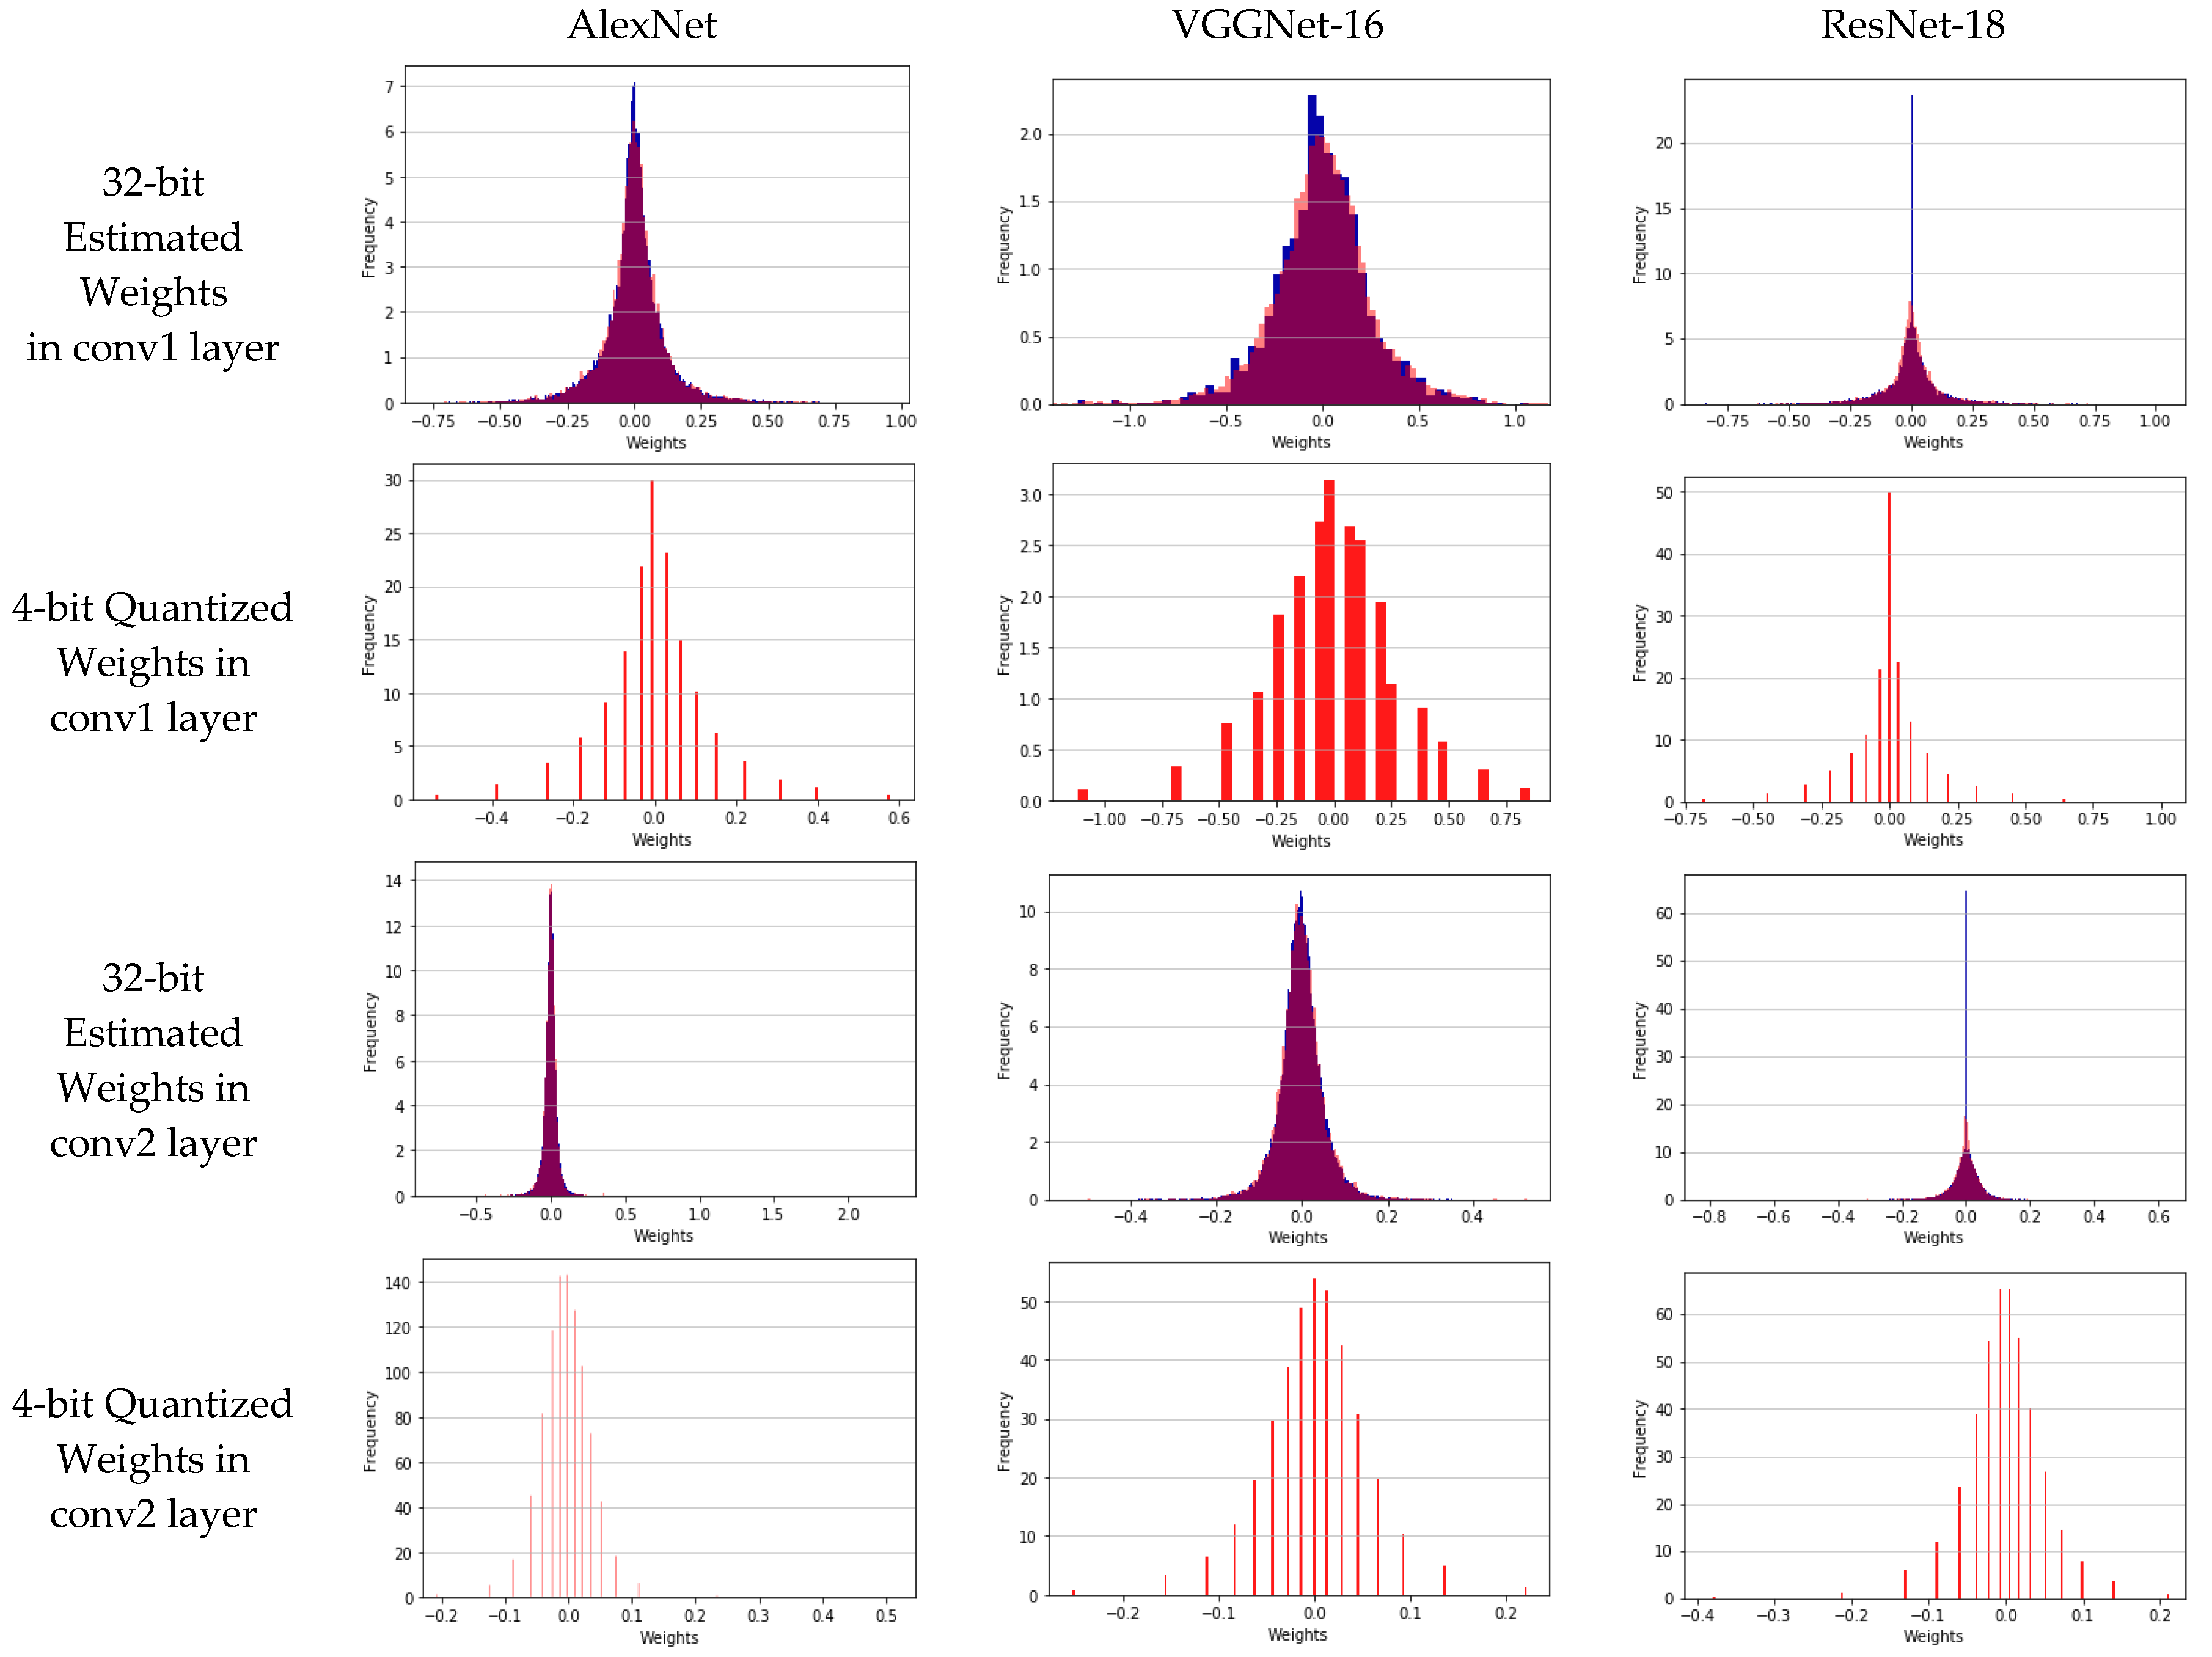
\includegraphics[height=0.8\textheight]{quantization} \\
    Image Source: \cite{seo_efficient_2019}
    \large
    SOTA: GPTQ \cite{frantar_gptq_2022}
    \pnote{
        quantization effectively reduces the resolutionof individual weights,
        and can be done while losing very little accuracy
    }
\end{frame}

\subsection{Distillation}
\begin{frame}[c]{Knowledge Distillation}
    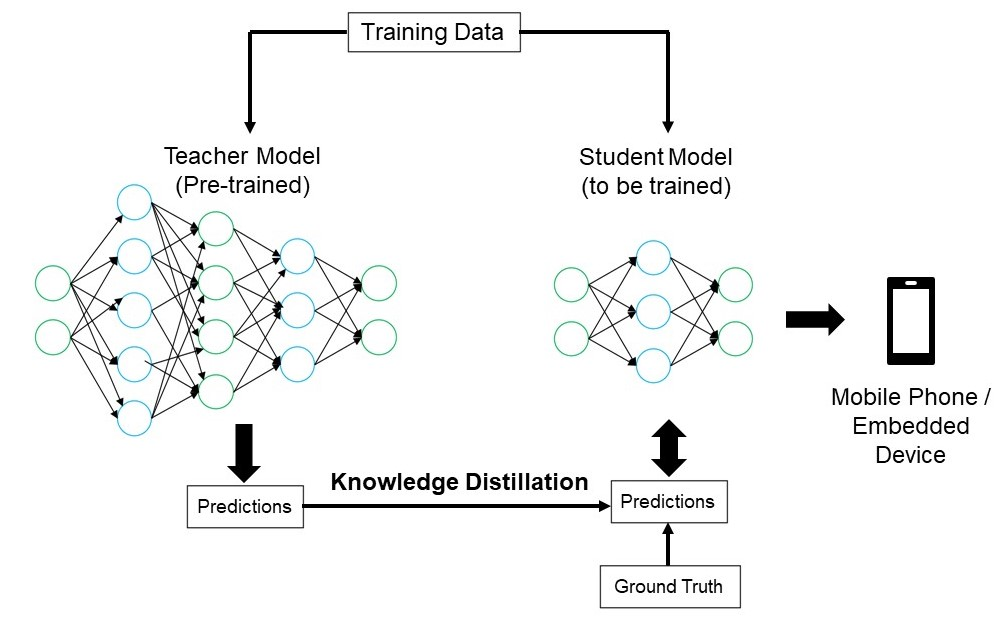
\includegraphics[width=\textwidth]{distillation} \\
    Image Source: \cite{gou_knowledge_2021}
\end{frame}
\begin{frame}[c]{Patient Knowledge Distillation}
    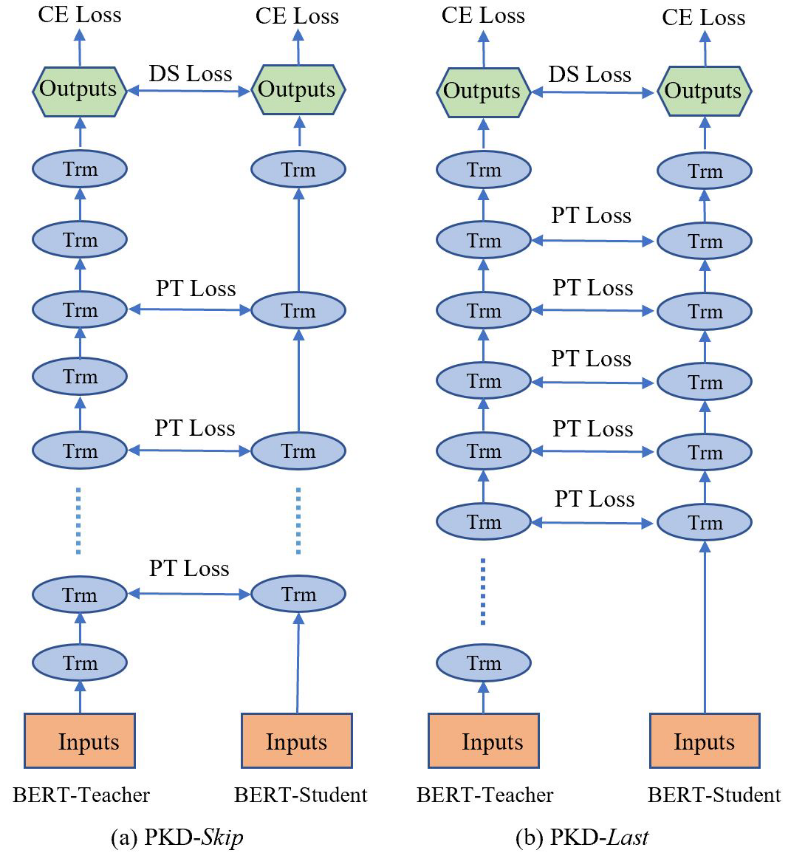
\includegraphics[height=0.8\textheight]{pkd} \\
    Image Source: \cite{sun_patient_2019}
\end{frame}

\subsection{Rank Reduction}
\begin{frame}[c]
    LoRA \cite{hu_lora_2021}
    (spun up for LlaMa just a month after 'release')
    \todo{use graphics from LoRA?}
\end{frame}

\subsection{Memorizing Transformer}
\begin{frame}[c]
    Memorizing \cite{wu_memorizing_2022}
    \todo{use loss curves?}
\end{frame}

\subsection{Reflexion}
\begin{frame}[c]{Reflexion}
    Reflexion \cite{rombach_highresolution_2022}
    \todo{use loss curves and architecture}
\end{frame}
